\hypersection{ch2703}{ポインターの内部実装}

ポインターの意味上と文法上の解説は終えた。ここからはポインターの内部実装\index{ぽいんた@ポインター!ないぶじつそう@内部実装}についてだ。ポインターの値とは外でもない、メモリー\index{めもり@メモリー}上のアドレス\index{あどれす@アドレス}のことだ。

\hypersubsection{ch270301}{キロバイトとキビバイト}

メモリーとアドレスについて解説する前に、キロバイト(Kilo byte)とキビバイト(Kibi byte)の違いについて解説する。
\index{きろばいと@キロバイト}\index{きびばいと@キビバイト}

キロ(Kilo)というのはSI接頭語\index{SI@SI接頭語}で、\(1000^1\)を意味する。1キロは1000だ。SI接頭語にはほかにもメガ(Mega, \(1000^2\))、ギガ(Giga, \(1000^3\))やテラ(Tera, \(1000^4\))などの接頭語もある。
\index{きろ@キロ}\index{めが@メガ}\index{ぎが@ギガ}\index{てら@テラ}

長さ1キロメートルは1000メートルで、重さ1キログラムは1000グラムだ。

いま「このCPUのクロック周波数は1GHzだ」と言ったとき、それは\(1000^3\)Hz = \(1000000000\)Hzのことだ。

しかし、メモリー容量だけは慣習的に\(1000^n\)ではなく、\(1024^n\)を使う。

一般人が「このメモリーは1KBだ」と言ったとき、それは1024バイトのことだ。1GBのメモリーは\(1024^3 バイト = 1073741824 バイト\)だ。筆者が本書を執筆するのに使ったラップトップコンピューターは32GBのメモリーを積んでいるがこれは34359738368バイトだ。

メモリーの容量が10進数ではなく2進数で数えられているのは、メモリーは2進数で扱うのがハードウェア的に都合がいいからだ。そのため、慣習的にキロは\(1000^1\)ではなく\(1024^1\)を意味するようになってしまった。

このため、IEEE 1541\index{IEEE 1541}では10進SI接頭語と対になる2進接頭語を定義した。

\ifTombow\pagebreak\fi
\begin{small}
\begin{longtable}[]{@{\,\,}ll@{\,\,}}
\hline%\toprule
\textsf{接頭語} & \textsf{値}\tabularnewline
\hline%\midrule
\endhead
キビ(kibi, Ki) & \(2^{10}\)\tabularnewline
メビ(mebi, Mi) & \(2^{20}\)\tabularnewline
ギビ(gibi, Gi) & \(2^{30}\)\tabularnewline
テビ(tebi, Ti) & \(2^{40}\)\tabularnewline
ペビ(pebi, Pi) & \(2^{50}\)\tabularnewline
エクスビ(exbi, Ei) & \(2^{60}\)\tabularnewline
\hline%\bottomrule
\end{longtable}
\end{small}

本書では1KBは1000バイトで、1KiBが1024バイトを意味する。

\hypersubsection{ch270302}{メモリーとアドレス}

コンピューターにはメモリー\index{めもり@メモリー}やストレージ\index{すとれじ@ストレージ}と呼ばれる記憶領域\index{きおくりよういき@記憶領域}がある。情報の最小単位はすでに学んだようにビット\index{びつと@ビット}だが、情報をビット単位で扱うのは不便なので、慣習的に複数の連続したビットを束ねたバイト\index{ばいと@バイト}という単位で扱っている。1バイトはほとんどのアーキテクチャで8ビットだ。メモリーは複数の連続したバイト列で成り立っている。

この連続したバイト列の中の任意の1バイトを指し示すのがアドレスだ。メモリーのバイト列の最初の1バイトのアドレスを0とし、次の1バイトアドレスを1とし、以降、その次を前のアドレスに1加えた値にしてみよう。

そのようなメモリーとアドレスのコンピューターでは、1バイトの符号なし整数で表現されたアドレスは、256バイトのメモリーの中の任意の1バイトをアドレスとして参照することができる。

これはとても抽象化された計算機で、現実の計算機はもっと複雑な実装になっている。しかしC++の規格としては、メモリーとはフラットな連続したバイト列であって、その任意の各バイトをアドレスから参照可能だという想定になっている。

アドレスが1バイトの符号なし整数で表現され、そのすべてのビットが使われる場合、256バイトの連続したメモリーをアドレス可能だ。

アドレスが2バイトならば、64KiBのメモリーをアドレス可能だ。

アドレスが4バイトならば、4GiBのメモリーをアドレス可能だ。

アドレスが8バイトならば、16EiBのメモリーをアドレス可能だ。

ポインターの値というのは、このアドレスの値のことだ。

\hypersubsection{ch270303}{ポインターのサイズ}
\index{ぽいんた@ポインター!さいず@サイズ}

ポインターの値というのはアドレスの値だ。ポインターの値を格納するのにもメモリーが必要だ。ではポインターのサイズは何バイトあるのだろう。

型\texttt{T}のサイズを調べるには\texttt{sizeof(T)}\index{sizeof(T)@\texttt{sizeof(T)}}を使う。

\begin{lstlisting}[language={C++}]
template <typename T >
void print_size()
{
    std::cout << sizeof(T) << "\n"s ;
}

int main()
{
    print_size<int *>() ;
    print_size<double *>() ;

    // ポインターへのポインター
    print_size<int **>() ; 
}
\end{lstlisting}

筆者の環境でこのプログラムを実行した結果は以下のようになった。

\begin{lstlisting}[style=terminal]
8
8
8
\end{lstlisting}

どうやら筆者の環境ではポインターのサイズはすべて8バイトらしい。

\hypersubsection{ch270304}{ポインターの値}
\index{ぽいんた@ポインター!あたい@値}

ポインターが8バイト、つまり64ビットの値であるならば、それを8バイトの符号なし整数として解釈した値はどうなるのだろう。

C++にはすべてのポインターの値を格納できるサイズの符号なし整数型が用意されている。\texttt{std::uintptr\_t}\index{uintptr\_t@\texttt{uintptr\_t}}だ。

\begin{lstlisting}[language={C++}]
int main()
{
    std::cout << sizeof( std::uintptr_t ) ;
}
\end{lstlisting}

筆者の環境でこのプログラムを実行した結果も\texttt{8}が出力される。

ポインターも\texttt{std::uintptr\_t}も8バイトだ。ポインターのバイト列を\texttt{std::uintptr\_t}として強引に解釈すれば、符号なし整数としての値を出力してみよう。

ある値\texttt{from}のバイト列を、同じバイト数のある型\texttt{to}の値として強引に解釈するC++20で追加された標準ライブラリに、\texttt{std::bit\_cast<to>(from)}\index{bit\_cast@\texttt{bit\_cast}}がある。

\begin{lstlisting}[language={C++}]
#include <bit>

int main()
{
    int data {} ;
    std::cout << std::bit_cast<std::uintptr_t>(&data) ;
}
\end{lstlisting}

\ifTombow\pagebreak\fi
このプログラムを何度か実行した結果、以下のような結果を得た。

\begin{lstlisting}[style=terminal]
$ make run
140725678382588
$ make run
140721510940268
$ make run
140731669632396
\end{lstlisting}

私の環境ではポインターの具体的な値は実行ごとに異なる。これは私の使っているOSがASLR(Address Space Layout Randomization)\index{ASLR(Address Space Layout Randomization)} を実装しているためだ。興味のある読者は調べてみるとよい。

この値は\texttt{int}型の変数\texttt{data}のポインターの整数としての値だ。このアドレスの場所に、\texttt{int}型のオブジェクトの最初の1バイトがあり、その次の場所に次の1バイトがある。

筆者の環境では\texttt{int}型は4バイトだ。

\begin{lstlisting}[language={C++}]
int main()
{
    std::cout << sizeof(int) ;
}
\end{lstlisting}

\texttt{int}型のオブジェクトは4バイトの連続したメモリー上に構築されている。つまり、本質的には以下のようなコードと同等になる。

\begin{lstlisting}[language={C++}]
int main()
{
    std::byte data[4] ;
    std::cout << std::bit_cast<std::uintptr_t>(&data[0]) ;
}
\end{lstlisting}

\texttt{std::byte}\index{byte@\texttt{byte}}というのは\texttt{sizeof(std::byte)}の結果が1になる、サイズが1バイトの符号なし整数型だ。

\texttt{std::byte}はC++で1バイトの生の値を表現するために使うことができる。配列は連続したバイト列なので、4バイトの\texttt{int}型は、本質的には上のようなコードになる。ただし上のコードはアライメントという概念が欠けている。これについてはあとで説明する。

ところで、\texttt{std::bit\_cast}は2020年に制定される国際標準規格C++20から入った。しかるに筆者がこの文章を書いているのは2018年だ。まだC++20を完全に実装したC++コンパイラーは存在しない。この本が出版されてしばらくは、読者の手元にもC++20コンパイラーは存在しないだろう。

\clearpage
\hypersubsection{ch270305}{std::bit\texttt{\_}castの実装}
\index{bit\_cast@\texttt{bit\_cast}}

ないものは自分で実装すればいい。\texttt{std::bit\_cast}に近いものを実装してみよう。

今回実装する\texttt{bit\_cast}は以下のような関数テンプレートだ。

\begin{lstlisting}[language={C++}]
template < typename To, typename From >
To bit_cast( From const & from )
{
    // 値fromのバイト列をTo型の値として解釈して返す。
}
\end{lstlisting}

\texttt{bit\_cast}の実装にはポインターが必要だ。\texttt{From}の値を表現するバイト列への先頭のポインターを取り、バイト単位で\texttt{To}の値を表現するバイト列にコピーすればよい。

標準ライブラリにはそのような処理を行ってくれる\texttt{std::memcpy(dest, src, n)}がある。ポインター\texttt{src}から\texttt{n}バイトをポインター\texttt{dest}から\texttt{n}バイトに書き込む関数だ。

\begin{lstlisting}[language={C++}]
template < typename To, typename From >
To bit_cast( From const & from )
{
    To to ;
    std::memcpy( &to, &from, sizeof(To) ) ;
    return to ;
}
\end{lstlisting}

これで\texttt{std::bit\_cast}の実装はできた。しかしこの実装は問題を\texttt{std::memcpy}にたらい回しにしただけだ。\texttt{std::memcpy}も実装できて初めて\texttt{std::bit\_cast}を自前で実装できたと言える。

\hypersubsection{ch270306}{std::memcpyの実装}
\index{memcpy@\texttt{memcpy}}

\texttt{std::memcpy}はC++コンパイラーによって効率のよいコードに置き換えられる。そのため自分で実装した\texttt{std::memcpy}を標準ライブラリと同じ効率にすることは難しいが、機能的にはほとんど同じものを作ることができる。

\texttt{memcpy}の実装にはポインターの詳細な理解が必要だ。

\texttt{std::memcpy}関数は以下のようになっている。

\begin{lstlisting}[language={C++}]
void * memcpy( void * dest, void const * src, std::size_t n )
{
    // srcの先頭バイトからnバイトを
    // destの先頭バイトからのバイト列にコピーし
    // destを返す
}
\end{lstlisting}

見慣れない\texttt{void *}\,\index{void *@\texttt{void *}}という型が出てきた。まずはこれについて学ぼう。

\hypersubsubsection{ch27030601}{void型}
\index{void@\texttt{void}}

\texttt{void}は特別な型だ。\texttt{void}型は何も値を持たない型という意味を持つ。例えば関数が戻り値を何も返さない場合、\texttt{void}型を返す関数として宣言される。

\begin{lstlisting}[language={C++}]
// 何も値を返さない関数
void f()
{
    // 何も値を返さない
    return ;
}
\end{lstlisting}

あらゆる値は\texttt{void}型に変換することができる。変換した結果は、何も値を持たない。

\begin{lstlisting}[language={C++}]
void f()
{
    return static_cast<void>(123) ;
}
\end{lstlisting}

C++17では、\texttt{void}型の変数は作れない。

\begin{lstlisting}[language={C++}]
// エラー
void x ;
\end{lstlisting}

ところで、読者が本書を読むころには、C++規格では\texttt{void}型の変数が作れるようになっているかもしれない。これは\texttt{void}型だけ変数を作れないのが面倒だから作れるようになるだけで、具体的な値のない変数になる。

\hypersubsubsection{ch27030602}{void *\,型}
\index{void *@\texttt{void *}}

\texttt{void *}\,型は「\texttt{void}型へのポインター型」だ。\texttt{int *}\,が「\texttt{int}型へのポインター型」であるのと同じだ。

\texttt{void *}\,型の値は、ある型\texttt{T}へのポインター型から型\texttt{T}という情報が消え去ったポインターの値だ。ポインターの値というのはアドレスで、アドレスというのは単なるバイト単位のメモリーを指す整数値だということを学んだ。\texttt{void *}\,型は特定の型を意味しないポインター型だ。

ある型\texttt{T}へのポインター型の値は、\texttt{void *}\,型に変換できる。

\begin{lstlisting}[language={C++}]
int main()
{
    int data { } ;

    // int *からvoid *への変換
    void * ptr = &data ;
}
\end{lstlisting}

\texttt{void *}\,型の値\texttt{e}から元の型\texttt{T}へのポインターに変換するには\texttt{static\_cast<T *>(e)}が必要だ。

\begin{lstlisting}[language={C++}]
int main()
{
    int data { } ;
    void * void_ptr = &data ;

    int * int_ptr = static_cast<int *>(void_ptr) ;
}
\end{lstlisting}

もし\texttt{static\_cast<T *>(e)}の\texttt{e}が\texttt{T *}\,として妥当なアドレスの値であれば、変換後も正しく動く。

\texttt{T const *}\,型は\texttt{void const *}\,型に変換できる。その逆変換もできる。

\begin{lstlisting}[language={C++}]
int main()
{
    int data {} ;
    int const * int_const_ptr = &data ;
    void const * void_const_ptr = int_const_ptr ;
    int const * original = static_cast<int const *>(void_const_ptr) ;
}
\end{lstlisting}

ポインター間の型変換で\texttt{const}を消すことはできない。

\texttt{memcpy}は\texttt{void *}\,を使うことで、どんなポインターの値でも取れるようにしている。C++にはテンプレートがあるので以下のように宣言してもよいのだが、
\begin{lstlisting}[language={C++}]
template < typename Dest, typename Src >
Dest * memcpy( Dest * dest, Src const * src, std::size_t n ) ;
\end{lstlisting}
\texttt{memcpy}はC++以前からあるC言語ライブラリなので、こうなっている。

\hypersubsubsection{ch27030603}{std::byte型}
\index{byte@\texttt{byte}}

\texttt{void *}\,型はアドレスだけを意味するポインター型なので、参照することができない。\texttt{memcpy}の実装にはポインターを経由して参照先を1バイトずつ読み書きする必要がある。そのための型として\texttt{std::byte}がある。

\texttt{std::byte}型は1バイトを表現するための型だ。\texttt{sizeof(std::byte)}の結果は\texttt{1}になる。

1バイトというのは10進数で\(0 \leqq n \leqq 255\)までの値を扱う。

\texttt{std::byte}はとても厳格に1バイトの符号なし整数として振る舞うので、普通の整数で初期化や代入をすることができない。

\begin{lstlisting}[language={C++}]
// エラー
std::byte a = 123 ;
std::byte b(123) ;

// これもエラー
a = 123 ;
\end{lstlisting}

\texttt{std::byte}に具体的な値で初期化するには\,\texttt{\{x\}}\,を使う。

\begin{lstlisting}[language={C++}]
std::byte a{123} ;
\end{lstlisting}

\texttt{std::byte}に値を代入するには\texttt{std::byte\{x\}}\,を使う

\begin{lstlisting}[language={C++}]
std::byte a ;
a = std::byte{123} ;
\end{lstlisting}

\texttt{static\_cast<std::byte>(x)}や\texttt{std::byte(x)}はコンパイルできるが、使ってはならない。

\begin{lstlisting}[language={C++}]
// 使ってはならない
std::byte a = static_cast<std::byte>(123) ;
std::byte b = std::byte(123) ;
\end{lstlisting}

なぜ使ってはならないかというと、範囲外の値を無理やり変換してしまうからだ。

\begin{lstlisting}[language={C++}]
std::byte a = static_cast<std::byte>(256) ;
std::byte b = std::byte(-1) ;
\end{lstlisting}

\hypersubsubsection{ch27030604}{配列のメモリー上での表現}
\index{はいれつ@配列!めもりじようでのひようげん@メモリー上での表現}

配列は要素型を表現するバイト列をメモリー上に連続して配置する。

例えば\texttt{int [3]}という配列があり、\texttt{sizeof(int)}が\texttt{4}の場合、全体で12バイトのメモリーが確保される。

\begin{lstlisting}[language={C++}]
int data[3] = {1,2,3} ;
\end{lstlisting}

最初の4バイト(0バイト目から3バイトまで)の領域は0番目の要素である\texttt{data[0]}で、その値は\texttt{1}だ。

次の4バイト(4バイト目から7バイト目まで)の領域は1番目の要素である\texttt{data[1]}で、その値は\texttt{2}だ。

最後の4バイト(8バイト目から11バイト目まで)の領域は2番目の要素である\texttt{data[2]}で、その値は\texttt{3}だ。

\begin{figure}[htbp]
  \centering
  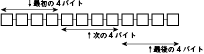
\includegraphics[scale=1.0]{fig/fig30-01.eps}
  \label{fig:30-01}
\end{figure}

実際にアドレスの生の値を出力して確かめてみよう。

\begin{lstlisting}[language={C++}]
// 生のアドレスを出力する関数
template < typename T >
void print_raw_address( T ptr )
{
    std::cout << std::bit_cast<std::uintptr_t>(ptr) << "\n"s ;
}

int main()
{
    int data[3] = {0,1,2} ;
    print_raw_address( &data[0] ) ;
    print_raw_address( &data[1] ) ;
    print_raw_address( &data[2] ) ;
}
\end{lstlisting}

このプログラムを筆者の環境で実行すると以下のように出力された。

\begin{lstlisting}[style=terminal]
140736120015884
140736120015888
140736120015892
\end{lstlisting}

筆者の環境では\texttt{sizeof(int)}は4だ。\texttt{\&data[0]}の生のアドレスに4を足した値が\,\texttt{\&data[1]}になっていることがわかる。

\hypersubsubsection{ch27030605}{ポインターと整数の演算}

ポインターと整数を加減算することができる。
\index{ぽいんた@ポインター!かげんざん@加減算}

ポインター\texttt{T *}\,に整数\texttt{n}を足すと、ポインターのアドレスが\texttt{sizeof(T) * n}加算される。この結果、ポインターは要素が配列のように配置された場合に\texttt{n}個先の要素を指すようになる。

\begin{lstlisting}[language={C++}]
template < typename T >
void print_raw_address( T ptr )
{
    std::cout << std::bit_cast<std::uintptr_t>(ptr) << "\n"s ;
}

int main()
{
    int a[4] = {0,1,2,3} ;

    // 0個目の要素へのポインター
    int * a0 = &a[0] ;
    print_raw_address( a0 ) ;
    

    // アドレスがsizeof(int) * 3加算される
    // a3は3個目の要素へのポインター
    int * a3 = a0 + 3 ;
    print_raw_address( a3 ) ;

    // アドレスがsizeof(int) * 2減算される。
    // a1は1個目の要素へのポインター
    int * a1 = a3 - 2 ;
    print_raw_address( a1 ) ;
}
\end{lstlisting}

これを筆者の環境で実行すると以下のように出力された。

\begin{lstlisting}[style=terminal]
140722117900224
140722117900236
140722117900228
\end{lstlisting}

最初の値が\texttt{a0}, 次の値が\texttt{a3}, 最後の値が\texttt{a1}だ。

筆者の環境では\texttt{sizeof(int)}は\texttt{4}だ。すると\texttt{a3}の値は\texttt{a0}の値より12多い値になっているはずだ。実際にそうなっている。\texttt{a1}は\texttt{a3}に対して8少ない値になっているはずだ。実際にそうなっている。

\hypersubsubsection{ch27030606}{いよいよmemcpyの実装}
\index{memcpy@\texttt{memcpy}}

これまで学んできたことをすべて使い、ようやく\texttt{memcpy}が実装できる。

\begin{enumerate}
\def\labelenumi{\arabic{enumi}.}
\item
  \texttt{dest}を\texttt{std::byte *}\,型に変換する
\item
  \texttt{src}を\texttt{std::byte const *}\,型に変換する
\item
  \texttt{src}の参照先から\texttt{n}バイトを\texttt{dest}の参照先にコピーする
\item
  \texttt{dest}を返す
\end{enumerate}

\begin{lstlisting}[language={C++}]
void * memcpy( void * dest, void const * src, std::size_t n )
{
    // destをstd::byte *型に変換
    auto d = static_cast<std::byte *>(dest) ;
    // srcをstd::byte const *型に変換する
    auto s = static_cast<std::byte const *>(src) ;

    // srcからnバイトコピーするのでnバイト先のアドレスを得る 
    auto last = s + n ;

    // nバイトコピーする
    while ( s != last )
    {
        *d = *s ;
        ++d ;
        ++s ;
    }

    // destを返す
    return dest ;
}
\end{lstlisting}

\hypersubsubsection{ch27030607}{memcpyの別の実装}

ポインターは\texttt{operator []}に対応している。
\index{[]@\texttt{[]}}

ポインター\texttt{p}と整数\texttt{i}に対して\texttt{p[i]}と書いたとき、\texttt{*(p + i)}という意味になる。

\begin{lstlisting}[language={C++}]
int main()
{
    int a[5] = {0,1,2,3,4} ;
    int * p = &a[0] ;

    p[0] ; // 0
    p[2] ; // 2

    int * p2 = &p[2] ;
    p2[1] ; // 3
}
\end{lstlisting}

\texttt{memcpy}は\texttt{operator []}を使って書くこともできる。

\begin{lstlisting}[language={C++}]
void * memcpy( void * dest, void const * src, std::size_t n )
{
    auto d = static_cast<std::byte *>(dest) ;
    auto s = static_cast<std::byte const *>(src) ;

    for ( std::size_t i = 0 ; i != n ; ++i )
    {
        d[i] = s[i] ;
    }

    return dest ;
}
\end{lstlisting}

\clearpage
\hypersubsection{ch270307}{データメンバーへのポインターの内部実装}
\index{でためんば@データマンバー!へのぽいんた@へのポインター}

データメンバーへのポインターの整数としての値は少し変わっている。

ポインターの生の値は、メモリー上で値を表現しているバイト列の先頭アドレスだ。

データメンバーへのポインターは、具体的なクラスのオブジェクトへのポインターやリファレンスがあって初めて意味がある。

\begin{lstlisting}[language={C++}]
struct S { int x = 123 ; } ;

int main()
{
    int data = 123 ;
    int * ptr = &data ;
    // ptr単体で参照できる
    int read1 = *ptr ;

    S object ;
    int S::* mem_ptr = &S::x ;
    // objectとmem_ptrの2つで参照できる
    int read2 = object.*mem_ptr ;

}
\end{lstlisting}

配列が要素型のバイト列を連続して配置したメモリーレイアウトをしているように、クラスもデータメンバーを連続して配置したメモリーレイアウトをしている。

たとえば以下のようなクラス\texttt{Object}がある場合、
\begin{lstlisting}[language={C++}]
struct Object
{
    int x ;
    int y ;
    int z ;
} ;
\end{lstlisting}
このクラスのサイズは\texttt{sizeof(Object)}だ。このクラスは\texttt{int}型のサブオブジェクトを3つ持っているので、そのサイズは少なくとも\texttt{size(int)*3}はある。

実際に確かめてみよう。

\begin{lstlisting}[language={C++}]
struct Object
{
    int x ;
    int y ;
    int z ;
} ;

int main()
{
    std::cout << "sizeof(int): " << sizeof(int) << "\n"s ;

    std::cout << "sizeof(Object): " << sizeof(Object) << "\n"s ;
}
\end{lstlisting}

このプログラムを筆者の環境で実行すると以下のように出力された。

\begin{lstlisting}[style=terminal]
sizeof(int): 4
sizeof(Object): 12
\end{lstlisting}

\texttt{int}型のサイズが\texttt{4}で、\texttt{Object}型のサイズが\texttt{12}ということは、クラス\texttt{Object}には\texttt{int}型のサブオブジェクトが3つ、\CID{1850}間なく連続して配置されているということだ。すべてのクラスがこうではないが、今回の私の環境ではそうなっている。

全体で12バイトということは、配列\texttt{int [3]}と同じように、最初の4バイトに\texttt{x}, \texttt{y}, \texttt{z}のどれかが、次の4バイトに残りのどちらかが、最後の4バイトに残りが配置されている。

データメンバーへのポインターというのは、このクラスのオブジェクトを表現するバイト列の先頭から何バイト目に配置されているかというオフセット値になっている。

具体的な値を見てみよう。

\begin{lstlisting}[language={C++}]
template < typename T >
void print_raw_address( T ptr )
{
    std::cout << bit_cast<std::uintptr_t>(ptr) << "\n"s ;
}

struct Object
{
    int x ;
    int y ;
    int z ;
} ;

int main()
{
    print_raw_address( &Object::x ) ;
    print_raw_address( &Object::y ) ;
    print_raw_address( &Object::z ) ;
}
\end{lstlisting}

\ifTombow\pagebreak\fi
このプログラムを筆者の環境で実行すると以下のように出力される。

\begin{lstlisting}[style=terminal]
0
4
8
\end{lstlisting}

筆者の環境では、\texttt{x}はクラスの先頭アドレスからオフセット0バイトに、\texttt{y}はオフセット4バイトに、\texttt{z}はオフセット8バイトに配置されているようだ。

確かめてみよう。

\begin{lstlisting}[language={C++}]
struct Object
{
    int x = 123 ;
    int y = 456 ;
    int z = 789 ;
} ;

int main()
{

    Object object ;

    // クラスのオブジェクトの先頭アドレス
    std::byte * start = bit_cast<std::byte *>(&object) ;
    // オフセット0
    int * x = bit_cast<int *>(start + 0) ;
    // オフセット4
    int * y = bit_cast<int *>(start + 4) ;
    // オフセット8
    int * z = bit_cast<int *>(start + 8) ;

    std::cout << *x << *y << *z ;
}
\end{lstlisting}

筆者の環境では以下のように出力される

\begin{lstlisting}[style=terminal]
123456789
\end{lstlisting}

このプログラムの実行結果は環境によって変わる。読者の使っている環境でデータメンバーへのポインターが筆者の環境と同じように実装されているとは限らない。
